\documentclass[tikz,dvisvgm,border=0pt]{standalone}
% Shared preamble of the diagrams in vignettes/articles/cuda-kernels.Rmd.
% Render them with `make diagrams` from the package root.
\usepackage[T1]{fontenc}
\usepackage{lmodern}
\usepackage{tikz}
\usetikzlibrary{arrows.meta, positioning, fit, backgrounds, calc, shapes.geometric, decorations.pathreplacing}

\definecolor{host}{HTML}{3B6EA8}
\definecolor{device}{HTML}{2E8B57}
\definecolor{accent}{HTML}{C0571B}
\definecolor{muted}{HTML}{6B6B6B}

% A white card behind every figure, so that it reads in pkgdown's dark mode.
\tikzset{
  every picture/.append style={
    show background rectangle,
    background rectangle/.style={fill=white, rounded corners=6pt},
    inner frame sep=8pt,
    font=\sffamily\small,
    >={Stealth[length=2.2mm]},
  },
  box/.style={draw, rounded corners=3pt, thick, align=center, inner sep=5pt, fill=white},
  hostbox/.style={box, draw=host, fill=host!8},
  devbox/.style={box, draw=device, fill=device!8},
  accbox/.style={box, draw=accent, fill=accent!8},
  region/.style={draw=#1, rounded corners=6pt, thick, dashed, inner sep=8pt},
  heading/.style={font=\sffamily\bfseries\small, text=#1},
  note/.style={font=\sffamily\footnotesize, text=muted, align=center},
  flow/.style={->, thick},
  code/.style={font=\ttfamily\footnotesize},
}

\begin{document}
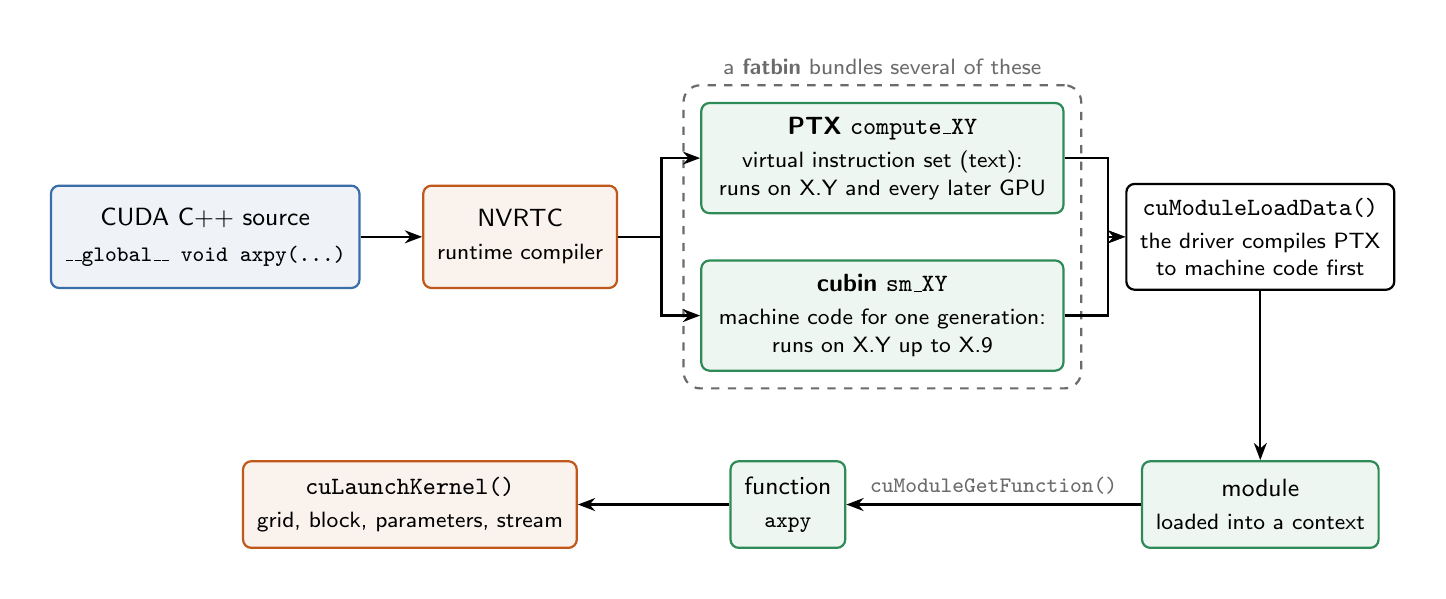
\begin{tikzpicture}
  \node[hostbox, minimum height=1.3cm] (src) at (0, 0)
    {CUDA C++ source\\[2pt]{\footnotesize\ttfamily \_\_global\_\_ void axpy(...)}};
  \node[accbox, minimum height=1.3cm] (nvrtc) at (4.0, 0) {NVRTC\\[1pt]{\footnotesize runtime compiler}};

  \node[devbox, minimum width=4.6cm] (ptx) at (8.6, 1.0)
    {\textbf{PTX} \texttt{compute\_XY}\\[1pt]{\footnotesize virtual instruction set (text):}\\[-1pt]{\footnotesize runs on X.Y and every later GPU}};
  \node[devbox, minimum width=4.6cm] (cubin) at (8.6, -1.0)
    {\textbf{cubin} \texttt{sm\_XY}\\[1pt]{\footnotesize machine code for one generation:}\\[-1pt]{\footnotesize runs on X.Y up to X.9}};
  \node[region=muted, fit=(ptx)(cubin), inner sep=6pt] (fat) {};
  \node[note, anchor=south] at (fat.north) {a \textbf{fatbin} bundles several of these};

  \node[box, minimum height=1.3cm] (load) at (13.4, 0)
    {\texttt{cuModuleLoadData()}\\[1pt]{\footnotesize the driver compiles PTX}\\[-1pt]{\footnotesize to machine code first}};

  \node[devbox, minimum height=1.1cm] (module) at (13.4, -3.4) {module\\[1pt]{\footnotesize loaded into a context}};
  \node[devbox, minimum height=1.1cm] (fn) at (7.4, -3.4) {function\\[1pt]{\footnotesize\ttfamily axpy}};
  \node[accbox, minimum height=1.1cm] (launch) at (2.6, -3.4)
    {\texttt{cuLaunchKernel()}\\[1pt]{\footnotesize grid, block, parameters, stream}};

  \draw[flow] (src) -- (nvrtc);
  \draw[flow] (nvrtc.east) -- ++(0.55, 0) |- (ptx.west);
  \draw[flow] (nvrtc.east) -- ++(0.55, 0) |- (cubin.west);
  \draw[flow] (ptx.east) -- ++(0.55, 0) |- (load.west);
  \draw[flow] (cubin.east) -- ++(0.55, 0) |- (load.west);
  \draw[flow] (load) -- (module);
  \draw[flow] (module) -- node[above, note] {\texttt{cuModuleGetFunction()}} (fn);
  \draw[flow] (fn) -- (launch);

\end{tikzpicture}
\end{document}
